% =====================================================================
%  CAI Assignment 2 report: Teach a Model When to Ask (LoRA + DPO)
%  ECE 6256 / CS 6604, Georgia Tech, Fall 2026
%
%  LIMIT: report body <= 3 pages. AI-use disclosure + references on page 4, figures after.
%  Build:  pdflatex A2_report && bibtex A2_report && pdflatex A2_report && pdflatex A2_report
% =====================================================================
\documentclass[11pt]{article}
\usepackage[final]{acl}
% tighter layout: smaller margins and title block
\geometry{margin=2cm}
\setlength\titlebox{3.4cm}
\usepackage{times}
\usepackage{latexsym}
\usepackage[T1]{fontenc}
\usepackage[utf8]{inputenc}
\usepackage{microtype}
\usepackage{graphicx}
\usepackage{booktabs}
\usepackage{amsmath,amssymb}
\usepackage{xcolor}
\usepackage[most]{tcolorbox}
\usepackage{enumitem}
\setlist{nosep,leftmargin=*}

\newcommand{\pp}{\,pp}

\newtcolorbox{transcript}[1]{enhanced, breakable, colback=gray!4, colframe=gray!55,
  boxrule=0.4pt, arc=1pt, left=3pt, right=3pt, top=1pt, bottom=1pt,
  fonttitle=\small\bfseries, title={#1}, fontupper=\footnotesize}
\newcommand{\usr}[1]{\textbf{User:} #1\par}
\newcommand{\base}[1]{\textbf{Base:} #1\par}
\newcommand{\dpo}[1]{\textbf{DPO ($\beta$=0.5):} #1\par}

\title{Teaching a 1B Instruct Model When to Ask:\\
LoRA SFT and a DPO $\beta$ Sweep for Clarification Behavior}

\author{Michael Incorvaia \\
  Georgia Institute of Technology \\
  \texttt{mincorvaia3@gatech.edu}}

\begin{document}
\maketitle

\begin{abstract}
Lets shift Llama-3.2-1B-Instruct so that it asks on underspecified requests and still answers when the request is clear, without giving up a 200-question MMLU slice.
From 2,600 seeds we build 2,805 preference pairs, warm-start a LoRA adapter with response-masked SFT, and run DPO at $\beta \in \{0.05, 0.1, 0.5\}$ with the frozen base model as the reference and an NLL anchor on the chosen response.
On our dev set (50 ambiguous, 50 clear), every DPO adapter clears the three targets.
At $\beta{=}0.5$, ask-rate rises from 54\% to 88\% ($+34$\pp), answer-rate falls from 98\% to 94\% ($-4$\pp), and MMLU moves from 41.0\% to 41.5\%.
The other two $\beta$ values clear the same targets. The MMLU gap between them is a handful of questions on this dev set.
Earlier recipes produced an over-asker (0\% answer-rate) and a forgetter (MMLU 26--30\%).
\end{abstract}

\section{Introduction}
\label{sec:intro}

Using the instruct models they often commit to a guess when a detail is missing.
A model that asks on every prompt is as broken as one that never asks, and a model that asks by forgetting how to emit a multiple-choice letter has not learned the behavior.
We fine-tune Llama-3.2-1B-Instruct \citep{grattafiori2024llama3} with LoRA \citep{hu2022lora} SFT and a three-value DPO sweep \citep{rafailov2023dpo}.
On a hand-written dev set, SFT already moves ask-rate from 54\% to 88\%. The $\beta$ differences on top of that sit inside the sampling noise of the dev set, which Section~\ref{sec:analysis} measures.
Section~\ref{sec:analysis} follows the two failures that forced the final data recipe.

\section{Preference Data}
\label{sec:data}

\paragraph{Construction.}
Llama-3.1-8B-Instruct, served with vLLM on PACE-ICE, writes the pairs.
Each of 2,600 seeds is a (domain, task, ambiguity, style, length-bucket) draw from a fixed RNG (seed 6604) of 48 domains, 17 task types, 8 ambiguity types, and three length buckets (short, medium, long).
One call returns a minimal pair, an underspecified request and a fully specified rewrite of the same task, plus a short name for the missing detail.
Four later calls write the responses for a specific clarifying question and a confident guess for the ambiguous prompt, a direct answer and a needless question for the clear prompt.
Topic and length are matched on the two sides, so the label has to track whether something is missing.
The ambiguous half of one generated minimal pair is in the training file as \texttt{pair\_001037}, kept as generated: ``Could you convert 25 meters to another unit so it's easier to measure long distances?'', the chosen response asks whether the unit should be yards, kilometers, or miles, and the rejected response guesses ``262.47 feet, 87.77 yards, 0.0277 miles, or 82.02 centimeters.''
The clear half is from the same generated minimal pair. It was dropped when the classes were balanced, so it is not in the training file: ``Convert 25 meters to yards with a precision of two decimal places and standard rounding conventions applied.'', the chosen response computes 27.40 yards, and the rejected response asks about the rounding rule the prompt already stated.

\paragraph{Filtering.}
Prompt filters (JSON, length, duplicates, overlap with the dev prompts) left 1,918 minimal pairs.
Response filters required a question mark on questions, none on answers, and a length bound, and the course judge had to agree with the intended ask/answer label.
That dropped 600 ambiguous and 17 clear pairs for format, and 171 ambiguous and 139 clear pairs because the judge disagreed.
We kept 2,246 pairs, 1,123 per class, balanced inside each length bucket.
A separate answerability check was near chance where we see that it called 40\% of ambiguous prompts unanswerable and 46\% of clear prompts answerable, so we logged it and did not filter on it.

Those 2,246 pairs still asked the 1B model to imitate 8B wording.
The final set replaces the chosen answer on 373 of the 1,123 clear prompts with the base 1B's own greedy decode (750 generations hit a 384-token cap and kept the 8B answer), and adds 259 self-contained Alpaca instructions, self-distilled the same way, plus 300 ARC letter-answer questions, which are not MMLU.
The training file is 2,805 pairs split into 1,123 ambiguous and 1,682 clear.

\paragraph{Hand verification.}
\texttt{sample\_for\_verification} draws 100 of the 8B pairs with \texttt{random.sample} at seed 6604 (44 ambiguous, 56 clear).
We marked each accept or reject in \texttt{tools/review\_pairs.py} for ones that were wrong class, chosen response no better than the rejected one, a vague question, or a poor answer.
We rejected 13/100.
Eleven of 44 ambiguous pairs (25\%) did not need a question; 2 of 56 clear pairs (3.6\%) were missing something real.
One ambiguous reject is ``Write a function to check if a string is a palindrome or not,'' reason ``not needed.''
One clear reject is a puppy-vaccine list whose question about breed was load-bearing (``breed is important'').
We kept those 13 rows. The sample is an audit of the 8B pairs, so dropping only the rows we read would leave that label error in the 8B pairs we did not read. A 13/100 count is about $\pm 7$ points wide, the same uncertainty Section~\ref{sec:analysis} gives the dev-set rates. The Alpaca, ARC, and self-distilled rows, about 930 of 2,805, were added or changed after this sample.

\section{Training}
\label{sec:training}

\paragraph{SFT-LoRA.}
The base is Llama-3.2-1B-Instruct.
LoRA uses $r{=}16$, $\alpha{=}32$, dropout 0.05 on \texttt{q,k,v,o\_proj}, with every base weight frozen at 3,407,872 trainable parameters, 0.275\% of 1,239,222,272.
SFT trains on the chosen response for 2 epochs (lr $10^{-4}$, batch 8, cosine decay, 5\% warmup, max length 1024, seed 42).
Cross-entropy is computed only on the final assistant turn.
Of 545,488 tokens, 336,900 (61.8\%) are supervised.
We checked the mask against the real Llama chat template; \texttt{setup.log} records \texttt{MASKING OK}.

\paragraph{DPO.}
DPO starts from that adapter and optimizes
\begin{equation}
\mathcal{L} = -\log\sigma\!\Big(\beta\big[\Delta_\theta(y_w) - \Delta_\theta(y_l)\big]\Big),
\label{eq:dpo}
\end{equation}
where $\Delta_\theta(y) = \log\pi_\theta(y\,|\,x) - \log\pi_{\mathrm{ref}}(y\,|\,x)$ is summed over response tokens.
We add $0.5$ times the length-normalized NLL of the chosen response.
The reference is the untouched instruct model, read with \texttt{disable\_adapter()} on the same weights, so the KL term pulls toward the original instruct model. The SFT adapter is only the initialization.
\texttt{sequence\_log\_prob} and \texttt{dpo\_loss} are implemented in \texttt{train\_dpo.py}.
Each $\beta \in \{0.05, 0.1, 0.5\}$ is its own adapter as 1 epoch, lr $10^{-5}$, micro-batch 4 pairs with gradient accumulation 2 (effective batch 8), 10\% warmup, max length 1024, seed 42.
The NLL weight is 0.5.
Earlier runs used a higher learning rate, a second epoch, and a zero or 0.2 anchor; Section~\ref{sec:analysis} says what those did.

\section{Results}
\label{sec:results}

Table~\ref{tab:main} is our dev set, not the hidden test set.
Ask-rate uses 50 hand-written ambiguous prompts, answer-rate 50 hand-written clear prompts, and MMLU a 200-question slice \citep{hendrycks2021mmlu} drawn with seed 6604.
The judge is the course Llama-3.1-8B-Instruct rubric \citep{zheng2023judging}, unmodified.
Each behavioral prompt moves a rate by 2 points, so 88\% is 44/50.
The graders will rerun \texttt{evaluate.py} on their own 150/150 split.

\begin{table}[t]
\centering
\small
\begin{tabular}{lccc}
\toprule
Model & Ask $\uparrow$ & Answer $\uparrow$ & MMLU \\
\midrule
Base             & 54 & 98 & 41.0 \\
SFT              & 88 & 94 & 38.0 \\
DPO $\beta$=0.05 & 88 & 98 & 38.0 \\
DPO $\beta$=0.1  & 88 & 96 & 38.5 \\
\textbf{DPO $\beta$=0.5} & \textbf{88} & \textbf{94} & \textbf{41.5} \\
\midrule
Target           & $\geq$79 & $\geq$93 & $\geq$38 \\
\bottomrule
\end{tabular}
\caption{Dev-set rates (\%). Targets are base $+25$\pp, base $-5$\pp, and within $3$\pp\ of base. Every DPO row clears all three. Bold is $\beta{=}0.5$, the point estimate whose MMLU matches the base. Section~\ref{sec:analysis} treats the gaps between $\beta$ values as within noise.}
\label{tab:main}
\end{table}

SFT already clears the three thresholds, with MMLU and answer-rate on the boundary.
DPO does not change the ask-rate count, while SFT and all three $\beta$ values are at 44 of 50.
SFT had already fit the asking behavior these pairs teach, so DPO has little left to move on this set.
The other 6 prompts are where a data ceiling, a judge mistake, or a real miss would show up. The rates do not say which.
$\beta{=}0.05$ has point estimates of 98\% answer-rate and 38.0\% MMLU; $\beta{=}0.5$ has 94\% and 41.5\%.
That is 2 clear prompts and 7 MMLU questions. We report $\beta{=}0.5$ because its MMLU point estimate sits on the base model, not because this dev set separates the two.

\section{Analysis}
\label{sec:analysis}

\begin{figure}[t]
\centering
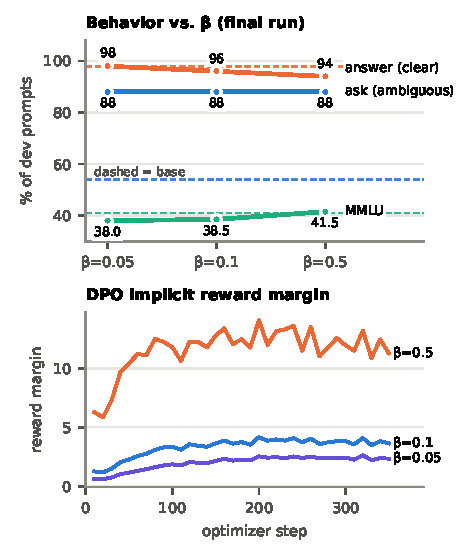
\includegraphics[width=0.86\columnwidth]{figs/beta_sweep.pdf}
\caption{$\beta$ sweep on the final run.
Top: ask-rate, answer-rate, and MMLU against $\beta$ (dashed lines are the base model).
Bottom: implicit reward margin over training.
Ask-rate is flat; the margin grows with $\beta$ because it is $\beta$ times the log-ratio gap.}
\label{fig:beta}
\end{figure}

\paragraph{The $\beta$ trade-off.}
On the final data the sweep does not trade ask-rate for retention.
Ask-rate is 88\% at every $\beta$ (Figure~\ref{fig:beta}, top).
The logged margin at step 350 is 2.3, 3.6, and 11.3 for $\beta = 0.05, 0.1, 0.5$.
(This kind of goes along with the weak/strong leash of the $\beta$ that we are constantly dealing with.) 
That ordering is the factor of $\beta$ in Equation~\ref{eq:dpo}.
Dividing by $\beta$ reverses it to about 46, 36, and 23. That larger gap at small $\beta$ is not a behavior difference this dev set can separate from noise.
A 95\% interval for an 88\% rate at $n{=}50$ is about 76--94\%, and the MMLU slice ($n{=}200$) is about $\pm 7$ points.
The 4-point answer-rate gap is 2 prompts, and the 3.5-point MMLU gap is 7 questions.

\paragraph{The over-asker.}
So, with the fact I did multiple runs in PACE
for v1 this built each pair in one JSON call, 
so the question was short and the answer was long, and length leaked the class.
DPO was plain with 2 epochs, lr $2{\times}10^{-5}$, NLL weight 0.
SFT asked on 100\% of ambiguous prompts and answered 40\% of clear ones.
DPO at $\beta{=}0.05$ answered 0 of 50 clear prompts, and $\beta{=}0.5$ answered 12\% (Figure~\ref{fig:fail} in the appendix).
v2 forced both prompts into the same length bucket.
SFT answer-rate went to 90\%, and $\beta{=}0.05$ still answered only 52\%.
The final run therefore uses one epoch, lr $10^{-5}$, and the NLL anchor.

\paragraph{The forgetter.}
That same v1, which didn't do so great, run dropped MMLU from 41.0\% to 26\% at $\beta{=}0.05$ and 30\% at $\beta{=}0.5$.
From step 10 to step 700, rejected log-probability fell from about $-46$ to about $-336$ and chosen log-probability from about $-38$ to about $-125$, with preference accuracy still above 0.96 (Figure~\ref{fig:dyn}).
So, though with v2, still imitating 8B answers, left SFT MMLU at 34.5\% and DPO at 27--29.5\%.
But when we moved to v3 copies in the base 1B's own clear answers and 300 ARC items, and MMLU returns to about 39--41\% while answer-rate stays at 82--88\%.
Until finally with v4's 259 Alpaca instructions bring the answer-rate to 94\%, and $\beta{=}0.5$ restores MMLU to 41.5\%.
On the final $\beta{=}0.05$ curve the log-probabilities stay near the start (about $-62/-93$ at step 10, about $-76/-132$ at step 350).
Data, epochs, learning rate, and the anchor all differ between those curves, so the flat v4 lines are the joint recipe (Figures~\ref{fig:fail} and \ref{fig:dyn}).

\section{Qualitative Transcripts}
\label{sec:transcripts}

Greedy decodes from the base model and the $\beta{=}0.5$ adapter. The base asks on 27 of 50 ambiguous prompts; SFT and every $\beta$ ask on 44 of 50.

\begin{transcript}{T1: ambiguous. Both ask. DPO asks only for the missing size.}
\usr{How much paint do I need for my room?}
\base{``I'll need to know a few details [\dots] 1.~Room size (in square feet) 2.~Room color 3.~Wall type 4.~Number of coats 5.~Any specific paint type.''}
\dpo{``[\dots] could you please specify the room's dimensions (length, width, and height) or the approximate square footage of the room?''}
\end{transcript}

\begin{transcript}{T2: clear. Both compute.}
\usr{What is 15\% of 240?}
\base{``240 * 0.15 = 36. The answer is 36.''}
\dpo{``240 * 0.15 = 36. So, 15\% of 240 is 36.''}
\end{transcript}

\begin{transcript}{T3: ambiguous. Base asks what the email is for. DPO drafts one anyway.}
\usr{Draft an email to my landlord.}
\base{``Before I start, could you please provide some details about the email? [\dots] the purpose of the email (e.g., rent payment, maintenance request, complaint).''}
\dpo{``I'll need to know more about the situation. Here's a general template [\dots] e.g.\ `The leaky faucet in the kitchen is causing water damage.'\,''}
\end{transcript}

\section{Conclusion}

We report $\beta{=}0.5$. This dev set cannot separate it from $\beta{=}0.05$, and the failure larger than that noise is the v1 collapse. T3 is the kind of miss that remains; some other no-question-mark outputs are still requests.

\section*{Reproducibility}

Adapters, the 2,805 pairs, and the hand audit are included. Seeds 6604 for data and eval, \verb|--seed 42| for training. See \texttt{REPRODUCE.md}.

\clearpage
\appendix
\section{AI-Use Disclosure}
\label{app:ai}

\paragraph{Data synthesis.}
Preference text was generated on PACE-ICE by Llama-3.1-8B-Instruct served with vLLM 0.11.0 (bf16, seed 6604); \texttt{gen\_v2.py} falls back to Hugging Face transformers only if vLLM fails to import, which did not happen in the final run.
The v4 generator is \texttt{gen\_v2.py}.
Stage A uses temperature 0.9 and top-$p$ 0.95 (system and user prompts \texttt{A\_SYS} / \texttt{A\_USR}); stage B uses temperature 0.7 for the four responses (\texttt{CLARIFY}, \texttt{GUESS}, \texttt{DIRECT}, \texttt{NEEDLESS}); the judge pass is greedy.
We drew 2,600 seeds.
Cached generations are \texttt{data/v2/A\_prompts.jsonl}, \texttt{B\_responses.jsonl}, and \texttt{C\_labels.jsonl}.
The earlier single-call generator's raw outputs are in \texttt{data/raw\_generations.jsonl}.
Quality control is the filter counts in Section~\ref{sec:data} and the 100-pair hand review, which we did ourselves in \texttt{tools/review\_pairs.py}.
Clear-prompt answers added later are greedy decodes of the base 1B (\texttt{tools/build\_v3.py}), not new 8B prose.
Alpaca and ARC contribute prompts and, for ARC, the gold letter.


\paragraph{Coding assistant.}
Claude (Anthropic) was used as a coding assistant to scaffold PACE scripts, implement and debug response masking and the DPO loss, and write the plotting scripts behind the figures.
We checked masking against the real chat template (\texttt{MASKING OK} in \texttt{setup.log}), ran the tiny-model smoke path, and read the loss, margin, and log-probability curves in the checkpoint logs before trusting a run.
The assistant was not used to write the analysis or results in this report.

\bibliography{A2_refs}

\onecolumn
\section{Failure-mode and DPO figures}
\label{app:figs}

\begin{figure}[h!]
\centering
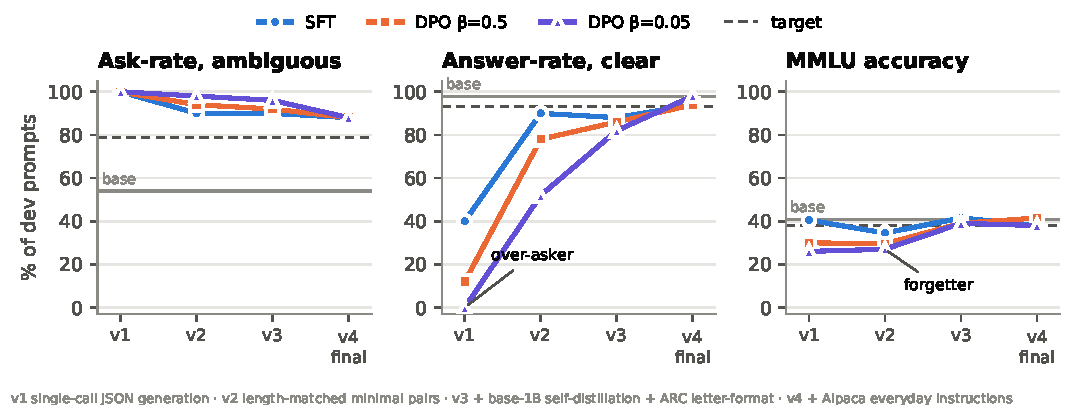
\includegraphics[width=\textwidth]{figs/fig2_failure_modes.pdf}
\caption{Dev-set ask-rate, answer-rate, and MMLU from v1 to v4, for SFT and for DPO at $\beta{=}0.05$ and $\beta{=}0.5$.
v1 answers almost no clear prompt.
v2 restores answering and loses MMLU.
v3 brings MMLU back.
v4 brings the answer-rate back over the target.}
\label{fig:fail}
\end{figure}

\begin{figure}[h!]
\centering
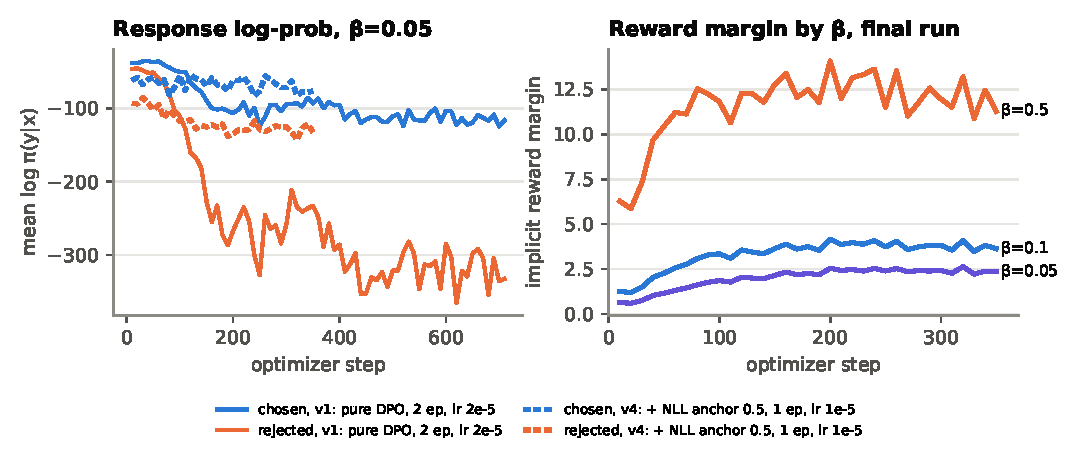
\includegraphics[width=\textwidth]{figs/fig3_dpo_dynamics.pdf}
\caption{DPO dynamics at the logged steps (the last point of each run is dropped; it averages fewer than 10 steps).
Left: at $\beta{=}0.05$, v1 drives the rejected log-probability from about $-46$ to about $-336$ and the chosen log-probability from about $-38$ to about $-125$.
v4, with one epoch, lr $10^{-5}$, and NLL weight 0.5, keeps both near the start.
Right: the $\beta$-scaled reward margin on the final run.}
\label{fig:dyn}
\end{figure}

\end{document}
